\documentclass[a4paper,12pt]{article}

\usepackage[utf8]{inputenc}
\usepackage[T1]{fontenc}
\usepackage[italian]{babel}
\usepackage{amsmath}
\usepackage{amssymb}
\usepackage{geometry}
\usepackage{graphicx}
\usepackage{hyperref}
\usepackage{titlesec}
\usepackage{parskip}
\usepackage{float}

% --- PACCHETTI PER CODICE PYTHON ---
\usepackage{listings}
\usepackage{xcolor}

% Definizione colori per il codice
\definecolor{codegreen}{rgb}{0,0.6,0}
\definecolor{codegray}{rgb}{0.5,0.5,0.5}
\definecolor{codepurple}{rgb}{0.58,0,0.82}
\definecolor{backcolour}{rgb}{0.95,0.95,0.92}

% Stile codice Python
\lstdefinestyle{mystyle}{
  backgroundcolor=\color{backcolour},
  commentstyle=\color{codegreen},
  keywordstyle=\color{magenta},
  numberstyle=\tiny\color{codegray},
  stringstyle=\color{codepurple},
  basicstyle=\ttfamily\footnotesize,
  breakatwhitespace=false,
  breaklines=true,
  captionpos=b,
  keepspaces=true,
  numbers=left,
  numbersep=5pt,
  showspaces=false,
  showstringspaces=false,
  showtabs=false,
  tabsize=2,
  language=Python
}
\lstset{style=mystyle}
% -----------------------------------

% Configurazione margini
\geometry{
  a4paper,
  total={170mm,257mm},
  left=25mm,
  top=25mm,
}

% Configurazione link
\hypersetup{
  colorlinks=true,
  linkcolor=black,
  filecolor=magenta,
  urlcolor=blue,
}

\title{}
\author{}

\begin{document}

% -------------------------------------------------------------------
% FRONTESPIZIO
% -------------------------------------------------------------------
\begin{titlepage}
\centering
\includegraphics[width=0.4\textwidth]{unica_800_black.png}\par
\vspace{1.5cm}
{\huge \textbf{Università degli Studi di Cagliari}\par}
\vspace{1cm}
{\Large Facoltà di Scienze\par}
{\Large Corso di Laurea Magistrale in Informatica\par}
\vspace{1.7cm}
{\Huge\bfseries Confronto di algoritmi di ottimizzazione di percorsi reali su rete stradale\par}
\vspace{1.5cm}
{\Large Applicazione del Branch-and-Cut per la risoluzione \\ del Traveling Salesman Problem \par}
\vspace{2cm}
\begin{minipage}{0.45\textwidth}
\begin{flushleft} \large
\textbf{Docente:}\\
Massimo \textsc{Di Francesco}
\end{flushleft}
\end{minipage}
\hfill
\begin{minipage}{0.45\textwidth}
\begin{flushright} \large
\textbf{Candidati:}\\
Salvatore Luigi Dettori \\
Mattia Piras
\end{flushright}
\end{minipage}

\vfill
{\large Anno Accademico 2024-2025\par}
\end{titlepage}

\tableofcontents
\newpage

% -------------------------------------------------------------------
\section{Introduzione}

Il problema del commesso viaggiatore (Traveling Salesman Problem o TSP) è uno dei problemi più noti e studiati nell'ambito della ricerca operativa e dell'ottimizzazione combinatoria.
La sfida consiste nel trovare il percorso più breve che permetta di visitare un insieme di luoghi esattamente una volta e ritornare al punto di partenza, tecnicamente definito come ciclo hamiltoniano.

In questa tesina viene analizzato un caso reale ambientato a Cagliari, in cui si vuole ottimizzare il percorso di un veicolo che rifornisce distributori di bevande in vari punti strategici (deposito, poli universitari, strutture ospedaliere) e in ulteriori punti di interesse dell’area metropolitana.
Per risolvere il problema viene implementato un algoritmo basato sul metodo \textbf{Branch-and-Cut}, che gestisce dinamicamente i vincoli di connettività (Subtour Elimination Constraints, SEC) sfruttando la struttura di un grafo stradale reale ottenuto tramite il servizio \texttt{OpenRouteService}.

% -------------------------------------------------------------------
\section{Approccio Teorico}

\subsection{Formulazione matematica del TSP}

Il TSP viene modellato come problema di Programmazione Lineare Intera su un grafo orientato \(G=(N,A)\), dove \(N\) è l’insieme dei nodi (località) e \(A\) l’insieme degli archi; a ciascun arco \((i,j)\) è associato un costo \(c_{ij}\) pari alla distanza stradale fra i due punti.  
Le variabili decisionali sono binarie e indicano la presenza dell’arco nel tour:
\[
x_{ij} =
\begin{cases}
1 & \text{se l'arco } (i,j) \text{ è incluso nel percorso}\\
0 & \text{altrimenti.}
\end{cases}
\]

La funzione obiettivo minimizza il costo totale:
\[
\min \sum_{(i,j)\in A} c_{ij} x_{ij},
\]
mentre i vincoli di grado impongono che ogni nodo abbia esattamente un arco entrante e uno uscente:
\[
\sum_{j\in N,\,j\neq i} x_{ij}=1 \quad \forall i\in N,
\qquad
\sum_{i\in N,\,i\neq j} x_{ij}=1 \quad \forall j\in N.
\]

\subsection{Connettività e vincoli SEC}

I soli vincoli di grado non garantiscono l’esistenza di un unico ciclo che copre tutti i nodi, poiché la soluzione può frammentarsi in più sottotour disgiunti.  
Per assicurare la connettività vengono introdotti i \textit{Subtour Elimination Constraints}:
\[
\sum_{(i,j)\in\delta^{+}(S)} x_{ij} \ge 1 \qquad \forall S\subset N,\,S\neq\emptyset,
\]
dove \(\delta^{+}(S)\) è l’insieme degli archi che escono da \(S\). 

Poiché il numero di sottoinsiemi \(S\) cresce esponenzialmente, tali vincoli non vengono generati tutti a priori, ma aggiunti \textit{on demand} tramite una procedura di separazione basata su problemi di Flusso Massimo / Taglio Minimo.

\subsection{Separazione tramite componenti fortemente connesse}

Il problema di separazione consiste nell’individuare, a partire da una soluzione \(\{x^*_{ij}\}\), se esiste un sottoinsieme \(S\) che viola un vincolo SEC.
L’approccio canonico della letteratura interpreta i valori \(x^*_{ij}\) come capacità e calcola un taglio minimo (Max-Flow / Min-Cut) per ogni coppia di nodi; se la capacità del taglio è inferiore a 1, l’insieme \(S\) definisce un vincolo SEC violato.

Nell’implementazione realizzata si adotta una strategia più semplice e diretta: il grafo di supporto viene costruito dagli archi con \(x^*_{ij}>0.01\) e si calcolano le \textbf{componenti fortemente connesse} (SCC) tramite la libreria \texttt{networkx}. Ogni componente \(S\) con \(1 < |S| < n\) individua un sottotour che viola il vincolo SEC corrispondente, il quale viene aggiunto al modello. Questo approccio è equivalente al Min-Cut sulle soluzioni intere (dove i valori sono in \(\{0,1\}\)) e si dimostra sufficientemente efficace anche sulle soluzioni frazionarie del rilassamento LP.

\newpage
% -------------------------------------------------------------------
\section{Implementazione Software}

\subsection{Definizione dei dati e matrici reali}

Lo script \texttt{tsp\_MTZ\_CS.py} definisce inizialmente l’elenco delle località come lista di dizionari contenenti nome, ID e coordinate geografiche in formato latitudine–longitudine.
Vengono considerati in totale 50 nodi.

Nel blocco principale il programma istanzia un oggetto \texttt{openrouteservice.Client} e richiama l’API \texttt{distance\_matrix} per ottenere sia le distanze sia le durate tra tutte le coppie di località, nel profilo \texttt{driving-car}. 
Le matrici risultanti, \texttt{dist\_matrix} e \texttt{dur\_matrix}, rappresentano rispettivamente i costi e i tempi di percorrenza che alimentano i modelli ILP.

\begin{lstlisting}[caption={Richiesta matrici reali tramite API OpenRouteService},label={lst:api}]
try:
    client = openrouteservice.Client(key=api_key)
    coords_for_api = [[loc["coords"][1], loc["coords"][0]] for loc in locations]
    matrix_response = client.distance_matrix(
        locations=coords_for_api,
        profile='driving-car',
        metrics=['distance', 'duration'],
        units='m'
    )
    dist_matrix = matrix_response['distances']
    dur_matrix = matrix_response['durations']
except Exception as e:
    print(f"Errore API: {e}")
    sys.exit(1)
\end{lstlisting}

\subsection{Formulazione Cut-Set e Branch-and-Cut}

La funzione \texttt{solve\_cutset\_with\_tracking} implementa la formulazione Cut-Set in tre step: rilassamento lineare, aggiunta iterativa dei tagli e soluzione intera finale.

\subsubsection*{Rilassamento lineare (Step 1)}

Nel primo step si costruisce un modello con variabili continue \(x_{ij}\in[0,1]\) e soli vincoli di grado, che rappresenta il rilassamento di assegnamento. 
La soluzione fornisce un bound inferiore iniziale e un tempo di calcolo dell’ordine di pochi centesimi di secondo, memorizzati in \texttt{step1\_lp\_bound} e \texttt{step1\_time}.

\subsubsection*{Aggiunta dei tagli (Step 2)}

Nel secondo step il rilassamento viene risolto più volte: a ogni iterazione viene costruito un grafo orientato di supporto dagli archi con $x^*_{ij}>0.01$ e si calcolano le \textbf{componenti fortemente connesse} (SCC) tramite \texttt{networkx.strongly\_connected\_components}. Ogni componente $S$ con $1<|S|<n$ individua un sottotour e il corrispondente vincolo SEC violato $\sum_{i\in S,\,j\notin S} x_{ij}\ge 1$ viene aggiunto al modello come \textit{user cut}. Il processo prosegue fino a quando non vengono trovate ulteriori violazioni o fino a un numero massimo di 15 iterazioni.

\subsubsection*{Soluzione intera (Step 3)}

Nello step finale viene risolto un modello intero con variabili binarie $x_{ij}$. Quando il solver trova una soluzione intera che contiene più cicli disgiunti, tali sottotour vengono individuati tramite SCC sul grafo degli archi selezionati e i corrispondenti vincoli SEC vengono aggiunti come \textit{lazy constraints}. In questo modo si ottiene un vero algoritmo Branch-and-Cut.
Al termine si ottiene un tour hamiltoniano unico: il codice ricostruisce la sequenza ordinata degli archi a partire dal nodo deposito fisico (\texttt{Deposito (Via S. Paolo)}, indice 0), calcola la distanza totale in metri (\texttt{step3\_integer\_solution}) e il tempo complessivo di percorrenza sommando le durate su ciascun arco (\texttt{final\_time}).

La funzione \texttt{solve\_cutset\_with\_callbacks} offre una variante che sfrutta le callback CPLEX (\textit{LazyConstraintCallback} e \textit{UserCutCallback}) per iniettare i vincoli SEC direttamente durante il Branch-and-Bound, riducendo il numero di nodi esplorati. Qualora le callback non siano disponibili nell'ambiente di esecuzione, la funzione ricade automaticamente in una modalità fallback che esegue lo stesso schema iterativo dello Step 3 descritto sopra.

\subsection{Formulazione MTZ}

La funzione \texttt{solve\_mtz} implementa la formulazione di Miller–Tucker–Zemlin, composta da un rilassamento continuo e da un modello intero con vincoli MTZ.
Nel rilassamento si introducono variabili di posizionamento \(u_i\in[0,n-1]\) e vincoli \(u_i - u_j + n x_{ij} \le n-1\) per tutti i nodi diversi dal deposito fisico (\texttt{Deposito (Via S. Paolo)}, indice 0), ottenendo un bound continuo alternativo rispetto alla formulazione a tagli. Il nodo deposito è escluso dai vincoli MTZ poiché funge da radice del tour e non richiede una variabile di ordinamento.

Per la soluzione intera, il modello MTZ viene ricostruito con variabili binarie e risolto con un limite di tempo di 300 secondi, registrando l’eventuale valore ottimo e il tempo necessario.
Nel caso con 50 nodi il bound continuo MTZ risulta di \(105\,204.98\) m, mentre la soluzione intera richiede l’intero time limit per raggiungere il valore dell’ottimo trovato con il Cut-Set.

\subsection{Visualizzazione geospaziale}

Per visualizzare il tour ottimo su mappa, lo script utilizza \texttt{geopandas}, \texttt{shapely} e \texttt{contextily}.
La funzione \texttt{plot\_solution\_on\_map} chiama per ogni arco ottimo l’API \texttt{directions} di OpenRouteService per recuperare la geometria stradale reale, che viene poi rappresentata come \texttt{LineString} su una basemap OpenStreetMap insieme ai punti delle località.

\begin{figure}[H]
\centering
\includegraphics[width=0.9\textwidth]{TSP_Map_CutSet_Final_50_Nodes.png}
\caption{Mappa del tour ottimo con 50 nodi ottenuto tramite formulazione Cut-Set.}
\label{fig:map_cutset}
\end{figure}

La Figura~\ref{fig:map_cutset} mostra il percorso ottimo di circa 127.63 km e 264 minuti che attraversa Cagliari, Quartu Sant’Elena e l’hinterland, con i nodi numerati in corrispondenza delle località principali.

\newpage
% -------------------------------------------------------------------
\section{Risultati Sperimentali}

\subsection{Confronto tra Cut-Set e MTZ}

Per confrontare le due formulazioni sono state costruite tabelle che riportano, per ogni metodo e fase, il bound ottenuto e il tempo di calcolo.
La Tabella~\ref{tab:confronto} evidenzia che il rilassamento Cut-Set fornisce un bound iniziale di 104701.11 m, migliorato a 125161.28 m dopo l’aggiunta dei tagli; l’ottimo intero raggiunge 127632.99 m in 0.7422 s con MIPGap nullo. La formulazione MTZ presenta un bound continuo di 105204.98 m e raggiunge lo stesso ottimo intero (127632.99 m) in 300.0653 s (al limite del time limit), esplorando 890795 nodi; a fine ricerca riporta BestBound = 124926.52 m e MIPGap = 2.12\%.

La variante \textbf{MTZ con radice virtuale} (\textit{Bastione Saint Remy}, indice~1) presenta un bound LP di 105254.85 m e raggiunge l’ottimo intero di 127632.99 m in 238.3109 s, esplorando soltanto 16681 nodi con un MIPGap residuo dello 0.01\%. Il confronto diretto con l’MTZ standard — stesso ottimo, $\sim$54× meno nodi esplorati, tempo ridotto del 21\% — conferma empiricamente che la scelta della radice influisce in modo determinante sull’efficienza della ricerca.

Per completezza, viene riportato anche il numero di nodi esplorati nell’albero di Branch-and-Bound, così da confrontare direttamente la dimensione della ricerca.
\begin{figure}[H]
\centering
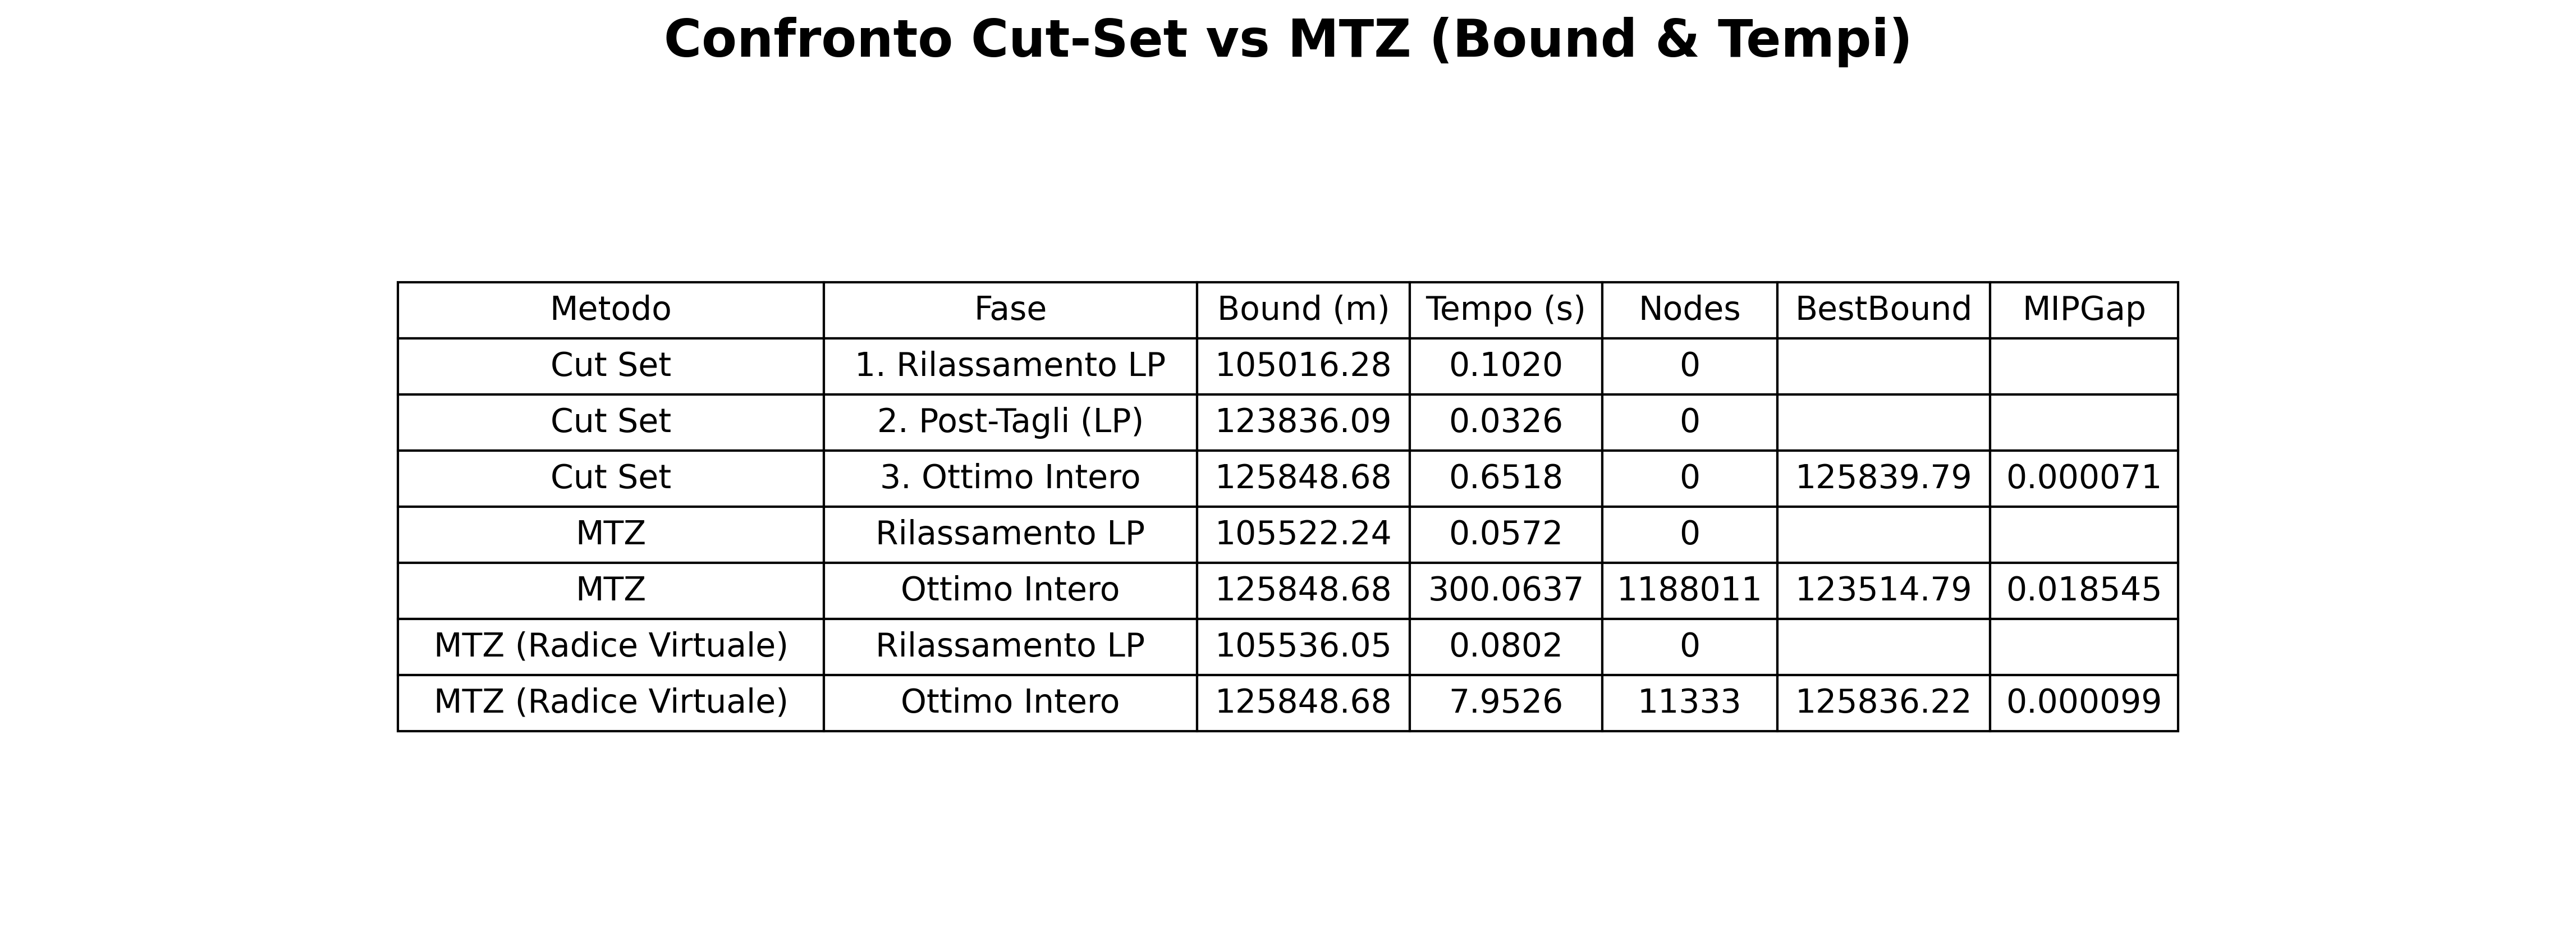
\includegraphics[width=0.95\textwidth]{Tabella_Confronto_Risultati.png}
\caption{Confronto tra formulazione Cut-Set e MTZ in termini di bound (m) e tempi di calcolo (s).}
\label{tab:confronto}
\end{figure}
\subsection{KPI Albero Branch-and-Bound}

Per valutare l’impatto dell’implementazione dei tagli sull’esplorazione dell’albero, sono state confrontate quattro configurazioni: (i) Cut-Set con aggiunta iterativa di SEC (\textit{loop cuts}), (ii) Cut-Set con \textit{lazy/user cuts} tramite callback, (iii) MTZ standard e (iv) MTZ con radice virtuale centrale.
I risultati in Figura~\ref{tab:kpi_bnb} mostrano che Cut-Set con \textit{lazy/user cuts} è la configurazione più veloce (0.5642 s, 212 nodi); la variante \textit{loop cuts} chiude all’origine (Nodes = 0) in 0.7422 s. L’MTZ standard raggiunge il time limit di 300.0653 s esplorando 890795 nodi. L’MTZ con radice virtuale (\textit{Bastione Saint Remy}) migliora sensibilmente: 238.3109 s e soli 16681 nodi, con MIPGap residuo dello 0.01\%, a conferma che la geometria della radice guida il solver verso l’ottimo in modo molto più efficiente.

\begin{figure}[H]
\centering
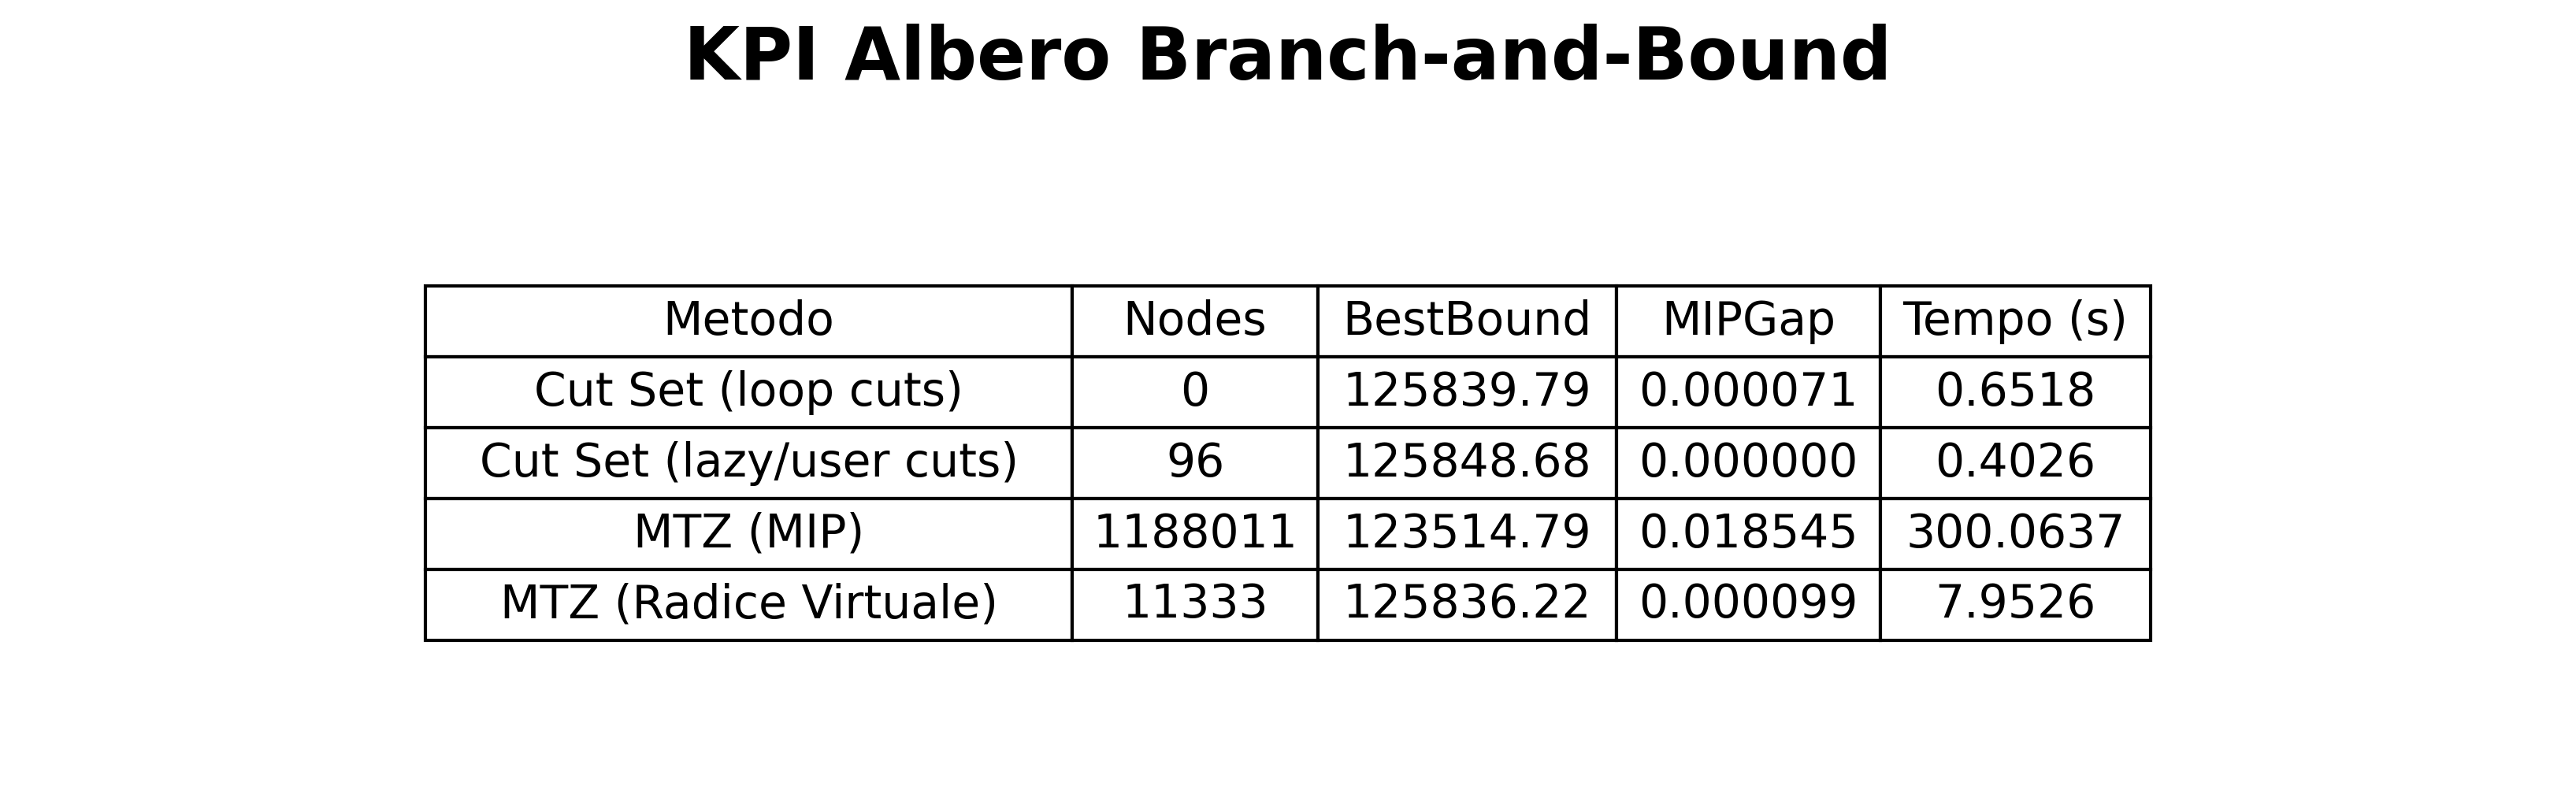
\includegraphics[width=0.85\textwidth]{Tabella_KPI_Albero_BnB.png}
\caption{KPI dell’albero di Branch-and-Bound per quattro configurazioni: Cut-Set (\textit{loop cuts}), Cut-Set (\textit{lazy/user cuts}), MTZ (MIP) e MTZ con radice virtuale.}
\label{tab:kpi_bnb}
\end{figure}


\subsection{Analisi dei GAP}

La qualità dei rilassamenti è stata misurata tramite il GAP percentuale rispetto all’ottimo intero Cut-Set, calcolato come
\[
\text{GAP} = \frac{z^{\text{int}} - z^{\text{LP}}}{z^{\text{int}}}\cdot 100,
\]
dove \(z^{\text{int}}\) è il valore ottimo intero e \(z^{\text{LP}}\) il bound continuo.  
La Tabella~\ref{tab:gap} mostra che il GAP iniziale dell’MTZ standard è pari a 17.57\%, quello dell’MTZ con radice virtuale è 17.53\% e quello iniziale del Cut-Set è 17.97\%; dopo l’aggiunta dei tagli il GAP del Cut-Set scende a 1.94\%, segnalando un rilassamento molto più stretto. I due rilassamenti MTZ sono quasi identici (differenza $<$ 0.05\%), confermando che la scelta della radice non altera la qualità del bound LP ma incide drasticamente sull’esplorazione dell’albero intero.

\begin{figure}[H]
\centering
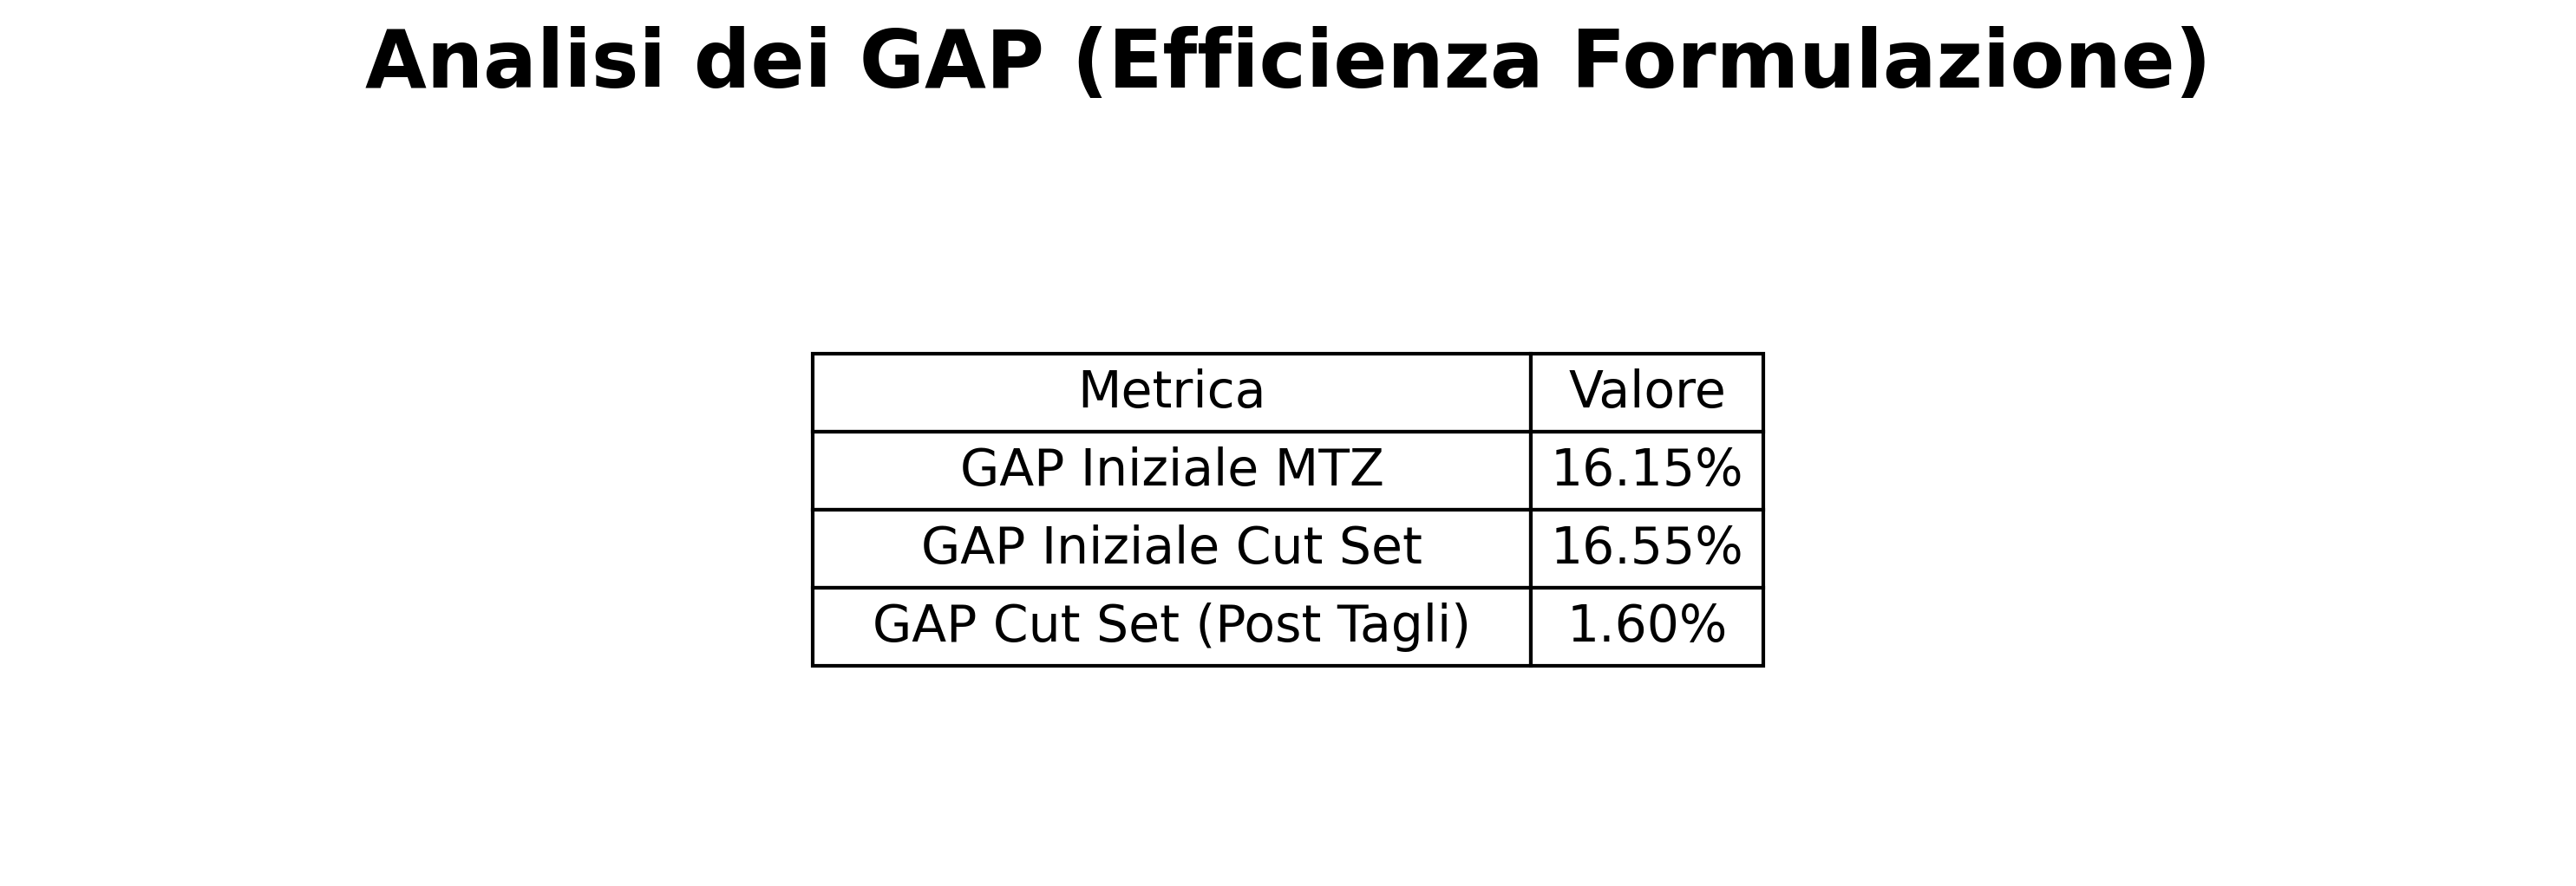
\includegraphics[width=0.7\textwidth]{Tabella_Gap_Analysis.png}
\caption{Analisi dei GAP percentuali delle formulazioni rispetto all’ottimo intero Cut-Set.}
\label{tab:gap}
\end{figure}

\newpage
% -------------------------------------------------------------------
\section{Analisi e Discussione}

\subsection{Caso di studio su Cagliari}

Le località considerate comprendono il deposito di partenza, diversi poli universitari, ospedali e punti di interesse dell’area metropolitana di Cagliari, fino a coprire 50 nodi complessivi. 
La mappa finale conferma che il tour ottimizzato segue la struttura reale della rete stradale, includendo i collegamenti principali verso Quartu Sant’Elena, l’area del Poetto e la zona industriale occidentale.  

\subsection{Valutazione delle prestazioni}

Dal confronto emerge che la formulazione Cut-Set parte da un rilassamento iniziale pari a 104701.11 m, ma grazie ai tagli il bound LP sale a 125161.28 m con un GAP residuo dell’1.94\% rispetto all’ottimo di 127632.99 m, raggiunto in 0.7422 s.
L’MTZ standard presenta un bound continuo di 105204.98 m e raggiunge lo stesso valore ottimo soltanto al termine del time limit (300.0653 s), esplorando 890795 nodi. L’MTZ con radice virtuale (\textit{Bastione Saint Remy}) produce lo stesso ottimo in 238.3109 s con soli 16681 nodi, dimostrando un miglioramento concreto ma insufficiente a colmare il divario con la formulazione Cut-Set.

\subsection{Anomalia rilevata: divergenza dei tempi MTZ}

Nel corso dello sviluppo è emersa un'anomalia significativa nei tempi di risoluzione della formulazione MTZ: una versione precedente dello script terminava in circa 8 secondi, mentre la versione attuale raggiunge sistematicamente il limite di 300 secondi senza confermare l'ottimalità.

\subsubsection*{Causa: il cambio di deposito}

L'analisi comparata delle due versioni del codice ha individuato la causa in un'unica modifica logica: il nodo di partenza del tour.

\begin{itemize}
  \item \textbf{Versione precedente:} il deposito implicito era il \textit{Bastione Saint Remy} (indice~1), un nodo geograficamente \textbf{centrale} rispetto all'insieme delle 50 località.
  \item \textbf{Versione attuale:} il deposito è stato correttamente fissato al \textit{Deposito (Via S.~Paolo)} (indice~0), un nodo \textbf{periferico} e asimmetrico rispetto alla maggior parte degli altri nodi.
\end{itemize}

Dal punto di vista implementativo, la differenza si riduce a come vengono esclusi i vincoli MTZ per il nodo deposito:

\begin{lstlisting}[caption={Vecchio codice: esclusione implicita del nodo 0},label={lst:mtz_old}]
for i in cities[1:]:   # esclude sempre l'indice 0
    for j in cities[1:]:
        if i != j:
            mdl_mtz.add_constraint(u[i] - u[j] + n*x[(i,j)] <= n-1)
\end{lstlisting}

\begin{lstlisting}[caption={Nuovo codice: esclusione esplicita del deposito reale},label={lst:mtz_new}]
cities_non_depot = [i for i in cities if i != depot_id]
for i in cities_non_depot:   # depot_id = 0
    for j in cities_non_depot:
        if i != j:
            mdl_mtz.add_constraint(u[i] - u[j] + n*x[(i,j)] <= n-1)
\end{lstlisting}

Sebbene i due frammenti siano logicamente equivalenti (il deposito occupa comunque la prima posizione nella lista), il cambio di coordinate modifica l'intera matrice delle distanze ORS e quindi la struttura dell'albero Branch-and-Bound che CPLEX deve esplorare.

\subsubsection*{Spiegazione tecnica: debolezza del rilassamento MTZ}

La formulazione MTZ introduce $O(n^2)$ vincoli di eliminazione dei sottotour già nel rilassamento LP:
\[
u_i - u_j + n\,x_{ij} \le n-1 \qquad \forall\,i,j \in V\setminus\{0\},\ i\neq j.
\]
Con $n=50$ questo equivale a circa 2\,400 vincoli aggiuntivi. Nonostante l'elevato numero di vincoli, il rilassamento continuo risultante è \textbf{debole}: il gap tra il bound LP e la soluzione intera ottima è ampio e fortemente dipendente dalla geometria dell'istanza. In presenza di un deposito periferico e di distanze asimmetriche, le euristiche interne del solver perdono efficacia, l'albero di Branch-and-Bound si espande in profondità e il tempo di risoluzione diventa altamente variabile, come sintetizzato di seguito:
\[
\text{Gap MTZ} \gg \text{Gap Cut Set}
\;\Rightarrow\;
\text{albero B\&B molto più profondo}
\;\Rightarrow\;
\text{tempo di risoluzione fino al timeout}.
\]
La formulazione Cut Set, al contrario, aggiunge vincoli SEC \textit{on demand}, soltanto sui sottotour effettivamente violati, mantenendo un bound LP molto più stretto e rendendo la ricerca robusta rispetto alla scelta del deposito.

\subsubsection*{Implicazioni pratiche}

Questo caso di studio evidenzia empiricamente una delle regole fondamentali dell'ottimizzazione su reti reali:
\begin{itemize}
  \item La formulazione \textbf{MTZ è instabile} e sensibile alla distribuzione geografica dei nodi; può risultare efficiente su istanze favorevoli ma non è affidabile per la messa in produzione.
  \item La formulazione \textbf{Cut Set (con callback CPLEX)} garantisce tempi ridotti e MIPGap nullo indipendentemente dalla posizione del deposito, ed è da preferire per problemi TSP e VRP su reti stradali reali.
\end{itemize}

\subsubsection*{Possibile mitigazione: nodo radice virtuale per MTZ}

Esiste tuttavia un modo per aggirare la debolezza dell'MTZ senza abbandonare la formulazione: sfruttare il fatto che un ciclo hamiltoniano \textbf{non ha un punto di partenza fisso}. La soluzione ottima del TSP è un anello chiuso; percorrerlo a partire dal nodo~A o dal nodo~B produce esattamente lo stesso insieme di archi e la stessa distanza totale.

Di conseguenza, è possibile impostare come \textit{radice virtuale} del modello MTZ un nodo \textbf{geograficamente centrale} — ad esempio il \textit{Bastione Saint Remy} (indice~1), che si trova al centro dell'area coperta dai 50 nodi — indipendentemente da quale sia il deposito operativo reale. Il solver trova la soluzione ottima in pochi secondi grazie alla geometria favorevole, e il tour restituito è identico in termini di archi e costo. In fase operativa, il veicolo parte semplicemente dal \textit{Deposito (Via S.~Paolo)} e percorre il ciclo ottimo a partire da quel nodo: poiché il percorso è un anello, ogni nodo del tour può fungere da punto d'ingresso senza alterare la soluzione.

\begin{figure}[H]
\centering
\begin{minipage}{0.85\textwidth}
\small
\textbf{Esempio:} supponiamo che il tour ottimo sia $A \to B \to C \to D \to A$. Se il modello MTZ ha calcolato questo ciclo usando $B$ come radice virtuale, il veicolo reale che parte da $C$ percorre semplicemente $C \to D \to A \to B \to C$: stessi archi, stesso costo, stesso ottimo.
\end{minipage}
\end{figure}

I risultati sperimentali ottenuti con questa tecnica confermano parzialmente l'ipotesi: l'MTZ con radice virtuale (\textit{Bastione Saint Remy}, indice~1) raggiunge l'ottimo di 127632.99 m in \textbf{238.3109 s}, esplorando soltanto \textbf{16681 nodi} con un MIPGap residuo dello \textbf{0.01\%}. A confronto, l'MTZ standard con radice nel \textit{Deposito (Via S.~Paolo)} impiega 300.0653 s (time limit) ed esplora 890795 nodi. Il guadagno è consistente ($\sim$54× meno nodi, $-$21\% sul tempo), ma non sufficiente a eguagliare il Cut-Set che chiude in 0.7422 s.

Questa tecnica permette quindi di \textbf{ridurre significativamente} il costo computazionale dell'MTZ, al costo di una sola modifica nel codice (il parametro \texttt{virtual\_root\_id} della funzione \texttt{solve\_mtz\_virtual\_root}). Rimane comunque una soluzione \textit{ad hoc} legata alla conoscenza a priori della geometria dell'istanza; la formulazione Cut Set resta preferibile ogni volta che tale conoscenza non è disponibile o la distribuzione dei nodi potrebbe cambiare nel tempo.

% -------------------------------------------------------------------
\section{Conclusioni}

Lo studio mostra come l’integrazione tra modelli di programmazione matematica, servizi cartografici online e librerie Python per l’ottimizzazione consenta di affrontare in modo efficace problemi logistici reali quali la pianificazione di un percorso di distribuzione su rete stradale.
La formulazione Cut-Set con schema Branch-and-Cut si dimostra particolarmente adatta al caso di studio: fornisce soluzioni ottime in tempi ridotti e permette di analizzare in modo dettagliato l’evoluzione del bound e dei sottotour, offrendo uno strumento flessibile per futuri ampliamenti del modello (vincoli di capacità, finestre temporali, più veicoli).

L’anomalia rilevata durante lo sviluppo — il passaggio da circa 8 secondi a oltre 300 secondi (time limit) per la formulazione MTZ a seguito del cambio di deposito — rafforza ulteriormente questa conclusione. Essa dimostra empiricamente che la scelta della formulazione non è indifferente rispetto ai dati di input: l’MTZ, pur corretto dal punto di vista teorico, espone un rilassamento continuo debole che lo rende suscettibile alla geometria dell’istanza.

La variante MTZ con radice virtuale centrale (\textit{Bastione Saint Remy}) ha prodotto un miglioramento misurabile — da 890795 a 16681 nodi esplorati, da 300 a 238 secondi — confermando che la scelta della radice orienta efficacemente le euristiche del solver. Tuttavia, il divario rispetto al Cut-Set (0.74 s, MIPGap nullo) rimane di due ordini di grandezza, a riprova che la tecnica della radice virtuale è un palliativo e non una soluzione strutturale. Per applicazioni reali su reti stradali con distribuzioni asimmetriche dei punti di consegna, la formulazione \textbf{Cut-Set con callback} rappresenta la scelta robusta e consigliata.

\end{document}
